\documentclass[10pt,aspectratio=169]{beamer}

% ─────────────────────────────────────────────────────────
% Theme & Colours
% ─────────────────────────────────────────────────────────
\usetheme{Madrid}
\usecolortheme{default}
\setbeamertemplate{navigation symbols}{}
\setbeamertemplate{footline}[frame number]

% ─────────────────────────────────────────────────────────
% Packages
% ─────────────────────────────────────────────────────────
\usepackage{amsmath,amssymb,amsthm}
\usepackage{mathtools}
\usepackage{graphicx}
\usepackage{booktabs}
\usepackage{xcolor}
\usepackage{tikz}
\usetikzlibrary{arrows.meta,positioning,shapes.geometric,calc}
\usepackage{subcaption}
\usepackage{array}
\usepackage{url}
\usepackage{hyperref}

% ─────────────────────────────────────────────────────────
% Custom Commands
% ─────────────────────────────────────────────────────────
\DeclareMathOperator{\divg}{div}
\DeclareMathOperator{\rot}{rot}
\newcommand{\norm}[1]{\left\|#1\right\|}
\newcommand{\R}{\mathbb{R}}
\newcommand{\myalert}[1]{\textcolor{red!70!black}{#1}}

% Colour boxes
\setbeamercolor{alertblock title}{bg=red!70!black, fg=white}
\setbeamercolor{alertblock body}{bg=red!10, fg=black}

% ─────────────────────────────────────────────────────────
% Title Info
% ─────────────────────────────────────────────────────────
\title[Hypercircle PINNs]{\textbf{Strict Error Control in Physics-Informed\\Neural Networks via the Hypercircle Method}}

\author[X.~Liu]{%
  \textbf{Xuefeng Liu}\\[2pt]
  {\small Tokyo Woman's Christian University}\\[4pt]
  {\footnotesize\itshape In collaboration with:}\\[1pt]
  {\footnotesize PingTing Hsieh \& ShengYao Huang}\\
  {\footnotesize (National Cheng Kung University, Taiwan)}%
}

\date{March 2026}

% ─────────────────────────────────────────────────────────
\begin{document}
% ─────────────────────────────────────────────────────────

% ====================================================
% SLIDE 1 – Title
% ====================================================
\begin{frame}
  \titlepage
\end{frame}

% ====================================================
% SLIDE 2 – Outline
% ====================================================
\begin{frame}{Outline}
  \tableofcontents
\end{frame}

% ====================================================
\section{Motivation}
% ====================================================

% ====================================================
% SLIDE 3 – Motivation
% ====================================================
\begin{frame}{Motivation: The Missing Guarantee in PINNs}

  \begin{columns}[T]
    \begin{column}{0.48\textwidth}
      \textbf{What PINNs promise}
      \begin{itemize}
        \item Mesh-free, flexible PDE solvers
        \item Works for forward \& inverse problems
        \item No geometry-dependent meshing
      \end{itemize}
      \bigskip
      \textbf{Two critical bottlenecks}
      \begin{enumerate}
        \item \textcolor{red!70!black}{\textbf{No certified error bound}}: residual
              is minimized \emph{statistically}; no
              rigorous guarantee on $\|u - v_{\theta}\|$
        \item \textcolor{red!70!black}{\textbf{Costly 2nd-order derivatives}}:
              computing $\Delta v$ via autograd is
              expensive \& exacerbates spectral bias
      \end{enumerate}
    \end{column}
    \begin{column}{0.48\textwidth}
      \begin{block}{Our Goal}
        Derive a \textbf{computable, strict}
        \emph{a posteriori} upper bound on the
        PDE approximation error — without knowing
        the exact solution $u$.
      \end{block}
      \bigskip
      \begin{block}{Key Idea}
        Revive the classical \textbf{Prager--Synge
        Hypercircle Theorem} (1947) and realise it
        via neural architectures that enforce
        admissibility \emph{by construction}.
      \end{block}
    \end{column}
  \end{columns}
\end{frame}

% ====================================================
\section{Problem Setup}
% ====================================================

% ====================================================
% SLIDE 4 – Problem Setup
% ====================================================
\begin{frame}{Problem Setup: Poisson Equation on Two Domains}

  \textbf{PDE:} Find $u$ such that
  \[
    -\Delta u = f \quad \text{in } \Omega, \qquad u = 0 \quad \text{on } \partial\Omega.
  \]

  \begin{columns}[T]
    \begin{column}{0.48\textwidth}
      \textbf{Domain 1 — Unit Disk}\\[4pt]
      $\Omega = \{(x,y) : x^2 + y^2 < 1\}$, $f \equiv 1$
      \[
        u_{\text{exact}} = \tfrac{1-r^2}{4},\quad
        \nabla u = \bigl(-\tfrac{x}{2}, -\tfrac{y}{2}\bigr)
      \]
      \textit{Smooth solution, classical benchmark.}

      \begin{center}
        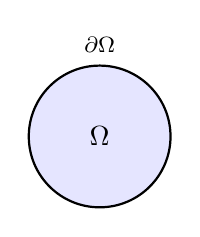
\begin{tikzpicture}[scale=0.9]
          \draw[thick,fill=blue!10] (0,0) circle (1.0);
          \node at (0,0) {$\Omega$};
          \node[above] at (0,1.05) {\footnotesize $\partial\Omega$};
        \end{tikzpicture}
      \end{center}
    \end{column}
    \begin{column}{0.48\textwidth}
      \textbf{Domain 2 — L-shaped Sector}\\[4pt]
      $\Omega = \{(r,\theta) : 0<r<1,\; 0<\theta<\tfrac{3\pi}{2}\}$
      \[
        u_{\text{exact}} = (r-1)^2 r^{2/3}\sin\!\bigl(\tfrac{2\theta}{3}\bigr)
      \]
      \textit{Re-entrant corner: gradient singular at $r=0$.}

      \begin{center}
        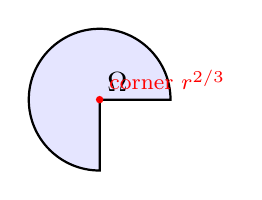
\begin{tikzpicture}[scale=0.9]
          \fill[blue!10]
            (0,0) -- (1,0) arc[start angle=0,end angle=270,radius=1] -- cycle;
          \draw[thick]
            (0,0) -- (1,0) arc[start angle=0,end angle=270,radius=1] -- cycle;
          \node at (0.25,0.25) {$\Omega$};
          \fill[red] (0,0) circle (1.5pt);
          \node[above right,red,font=\footnotesize] at (0,0)
            {corner $r^{2/3}$};
        \end{tikzpicture}
      \end{center}
    \end{column}
  \end{columns}
\end{frame}

% ====================================================
\section{Hypercircle Theorem}
% ====================================================

% ====================================================
% SLIDE 5 – Hypercircle Identity
% ====================================================
\begin{frame}{The Prager--Synge Hypercircle Theorem}

  Define two \textbf{admissible sets} in the Hilbert space $L^2(\Omega)^2$:

  \begin{columns}[T]
    \begin{column}{0.48\textwidth}
      \begin{block}{Kinematically Admissible $\mathcal{K}$}
        $v \in H^1_0(\Omega)$: satisfies Dirichlet BC
        \[
          v = 0 \text{ on } \partial\Omega
        \]
      \end{block}
    \end{column}
    \begin{column}{0.48\textwidth}
      \begin{block}{Statically Admissible $\mathcal{S}$}
        $\mathbf{p} \in H(\divg;\Omega)$: satisfies equilibrium
        \[
          \divg\mathbf{p} = -f \text{ in } \Omega
        \]
      \end{block}
    \end{column}
  \end{columns}
  \bigskip

  \textbf{Orthogonality:} For any $v\!\in\!\mathcal{K}$,
  $\mathbf{p}\!\in\!\mathcal{S}$, Green's identity gives
  \[
    \langle \nabla v - \nabla u,\; \mathbf{p} - \nabla u \rangle
    = -\!\int_\Omega (v-u)\underbrace{\divg(\mathbf{p}-\nabla u)}_{=0}\,d\Omega = 0.
  \]

  \begin{alertblock}{Hypercircle Identity (Pythagorean Theorem in $L^2$)}
    \[
      \underbrace{\norm{\nabla v - \mathbf{p}}^2}_{\textbf{Gap}^2 \;(\text{computable!})}
      \;=\;
      \underbrace{\norm{\nabla v - \nabla u}^2}_{\text{Primal Error}^2}
      +\;
      \underbrace{\norm{\mathbf{p} - \nabla u}^2}_{\text{Dual Error}^2}
    \]
    $\Rightarrow\quad \norm{\nabla v - \nabla u} \;\le\; \norm{\nabla v - \mathbf{p}}$
    \quad \textbf{(strict, computable upper bound)}
  \end{alertblock}
\end{frame}

% ====================================================
% SLIDE 6 – Geometric Picture
% ====================================================
\begin{frame}{Geometric Interpretation: The Hypercircle}

  \begin{columns}[T]
    \begin{column}{0.52\textwidth}
      \begin{center}
      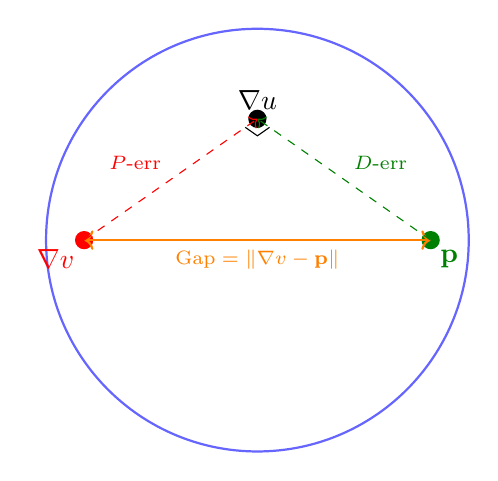
\begin{tikzpicture}[scale=2.2]
        % Hypercircle (circle with diameter GP)
        \coordinate (G) at (0,0);   % nabla v
        \coordinate (P) at (2,0);   % p
        \coordinate (U) at (1,0.7); % nabla u (on circle)
        \coordinate (C) at (1,0);   % centre

        \draw[thick,blue!60] (C) circle (1.22);

        % Points
        \fill[red]   (G) circle (1.5pt) node[below left] {$\nabla v$};
        \fill[green!50!black] (P) circle (1.5pt) node[below right] {$\mathbf{p}$};
        \fill[black] (U) circle (1.5pt) node[above] {$\nabla u$};

        % Gap = diameter
        \draw[thick,orange,<->] (G) -- (P)
          node[midway,below,font=\scriptsize]{$\text{Gap} = \norm{\nabla v - \mathbf{p}}$};

        % Primal error
        \draw[dashed,red,->] (G) -- (U)
          node[midway,above left,font=\scriptsize]{$P$-err};

        % Dual error
        \draw[dashed,green!50!black,->] (P) -- (U)
          node[midway,above right,font=\scriptsize]{$D$-err};

        % Right angle at u
        \draw[thin] ($(U)!0.07!(G)$) -- ($(U)!0.07!(G) + ($(U)!0.07!(P)$) - (U)$)
                    -- ($(U)!0.07!(P)$);
      \end{tikzpicture}
      \end{center}
    \end{column}
    \begin{column}{0.44\textwidth}
      \textbf{Key insight:}
      \begin{itemize}\setlength\itemsep{6pt}
        \item $\nabla u$ lies on a \emph{hypersphere}
              (circle in 2-D) whose diameter is the
              segment $[\nabla v,\, \mathbf{p}]$
        \item The right-angle at $\nabla u$ follows
              from orthogonality
        \item The diameter $\norm{\nabla v - \mathbf{p}}$
              is an \textbf{upper bound} for both
              primal and dual errors
        \item \textbf{No knowledge of $u$ needed}
              to evaluate the bound!
      \end{itemize}
    \end{column}
  \end{columns}
\end{frame}

% ====================================================
\section{Function Spaces: PINN vs.\ FEM}
% ====================================================

% ====================================================
% SLIDE 7 – Function Space Comparison
% ====================================================
\begin{frame}{Function Spaces: PINN vs.\ Classical FEM}

  \begin{center}
  \renewcommand{\arraystretch}{1.35}
  \small
  \begin{tabular}{@{}lll@{}}
    \toprule
    \textbf{Property}
      & \textbf{Classical FEM}
      & \textbf{PINN (this work)} \\
    \midrule
    \multicolumn{3}{@{}l}{\textit{Primal space (trial functions for $u$)}} \\
    \quad Space
      & $V_h \subset H^1_0(\Omega)$, piecewise polynomial
      & $\mathcal{N}_v \cdot d(\mathbf{x})$, globally $C^\infty$ \\
    \quad BC satisfaction
      & Nodal interpolation / strong imposition
      & \textbf{Exact}: $v = d(\mathbf{x})\,\mathcal{N}_v$,
        $d|_{\partial\Omega}=0$ \\
    \quad Approximation
      & Local (mesh-based), $O(h^k)$ convergence
      & Global (mesh-free), width/depth controlled \\
    \quad Regularity
      & $H^1$ (potentially discontinuous gradient)
      & $C^\infty$ (smooth activations like $\tanh$) \\
    \midrule
    \multicolumn{3}{@{}l}{\textit{Dual space (flux field $\mathbf{p}$)}} \\
    \quad Space
      & Raviart--Thomas $RT_k \subset H(\divg;\Omega)$
      & $\mathbf{p}_p + \rot(\mathcal{N}_\phi)$, globally $C^\infty$ \\
    \quad $\divg\mathbf{p}=-f$
      & Exactly at element level (RT property)
      & \textbf{Exact}: $\divg(\rot(\cdot))\equiv 0$ by identity \\
    \quad Construction
      & Complex: local Neumann problems / patch recovery
      & Simple: one scalar NN + autograd \\
    \quad Regularity
      & Piecewise, $H(\divg)$ only
      & $C^\infty$ flux field \\
    \midrule
    \multicolumn{3}{@{}l}{\textit{Error bound}} \\
    \quad Hypercircle bound
      & Requires expensive flux equilibration (Ainsworth--Oden)
      & \textbf{Direct}: minimise $\norm{\nabla v - \mathbf{p}}^2$ \\
    \quad Training cost
      & Solve linear system ($O(N^3)$ dense or iterative)
      & Stochastic gradient, first-order only \\
    \bottomrule
  \end{tabular}
  \end{center}

  \medskip
  \small
  \textbf{Key advantage}: Neural networks give $C^\infty$ approximation
  \emph{and} allow exact admissibility via architecture design —
  bypassing the mesh-complexity of RT elements.
\end{frame}

% ====================================================
\section{Admissible Neural Architectures}
% ====================================================

% ====================================================
% SLIDE 8 – Primal Network
% ====================================================
\begin{frame}{Primal Network: Kinematic Admissibility by Design}

  \textbf{Goal:} ensure $v \in H^1_0(\Omega)$,
  i.e.\ $v = 0$ exactly on $\partial\Omega$.

  \begin{columns}[T]
    \begin{column}{0.55\textwidth}
      \textbf{Hard boundary condition via distance mask:}
      \[
        v(\mathbf{x}) = d(\mathbf{x}) \cdot \mathcal{N}_v(\mathbf{x};\theta)
      \]
      \begin{itemize}
        \item $d(\mathbf{x})$ vanishes on $\partial\Omega$ analytically
        \item Regardless of weights $\theta$: $v|_{\partial\Omega} = 0$
        \item $\mathcal{N}_v$: fully-connected, $2\!\to\!50\!\to\!50\!\to\!1$, $\tanh$
      \end{itemize}

      \bigskip
      \textbf{Distance masks used:}
      \begin{align*}
        d_{\text{disk}}(\mathbf{x}) &= 1 - x^2 - y^2 \\
        d_{\text{sector}}(\mathbf{x}) &= (1-r)\,\theta\,({\textstyle\frac{3\pi}{2}}-\theta)
      \end{align*}
    \end{column}
    \begin{column}{0.42\textwidth}
      \begin{block}{Admissibility Verification}
        $v = d \cdot \mathcal{N}_v \;\Rightarrow$
        \begin{itemize}
          \item BC: $v|_{\partial\Omega} = 0$ \checkmark
          \item Regularity: $d$ bounded,
                $\mathcal{N}_v \in C^\infty$
                $\Rightarrow v \in H^1(\Omega)$ \checkmark
          \item \textbf{Conclusion:} $v \in \mathcal{K}$
        \end{itemize}
      \end{block}
      \medskip
      \begin{block}{Note on Regularity}
        With $\tanh$ activations, $\mathcal{N}_v$
        is $C^\infty$. Multiplied by smooth $d$,
        $v$ is smoother than any FEM piecewise
        polynomial.
      \end{block}
    \end{column}
  \end{columns}
\end{frame}

% ====================================================
% SLIDE 9 – Dual Network
% ====================================================
\begin{frame}{Dual Network: Static Admissibility by Design}

  \textbf{Goal:} ensure $\divg\mathbf{p} = -f$ \emph{exactly in $\Omega$}.

  \begin{columns}[T]
    \begin{column}{0.55\textwidth}
      \textbf{Decomposition:}
      \[
        \mathbf{p} = \underbrace{\mathbf{p}_p}_{\divg\mathbf{p}_p = -f}
                   + \underbrace{\rot(\mathcal{N}_\phi)}_{\divg(\rot(\cdot))\equiv 0}
      \]
      where $\rot(\phi) = \bigl(\partial_y\phi,\;-\partial_x\phi\bigr)$.

      \bigskip
      \textbf{Particular solutions:}
      \begin{itemize}
        \item Disk ($f=1$):
              $\mathbf{p}_p = (-\tfrac{x}{2}, -\tfrac{y}{2})$ \;(analytical)
        \item Sector (singular $f$):
              $\mathbf{p}_p = \sin(\tfrac{2\theta}{3})\bigl(2.5r^{5/3} - 2.8r^{2/3}\bigr)
              (\cos\theta, \sin\theta)$
      \end{itemize}
    \end{column}
    \begin{column}{0.42\textwidth}
      \begin{block}{Admissibility Verification}
        \[
          \divg\mathbf{p} = \underbrace{\divg\mathbf{p}_p}_{=-f}
                          + \underbrace{\divg(\rot\phi)}_{=0} = -f
        \]
        Holds \textbf{algebraically}, for any $\theta$.
      \end{block}
      \medskip
      \begin{block}{Why curl works}
        Vector identity: $\divg(\rot(\phi)) \equiv 0$
        for any differentiable $\phi$.
        \\[4pt]
        Same principle as \emph{mimetic} / div-free
        finite element formulations.
      \end{block}
    \end{column}
  \end{columns}

  \bigskip
  \textbf{Network:} $\mathcal{N}_\phi$: $2\!\to\!50\!\to\!50\!\to\!1$, $\tanh$;
  gradients via autograd $\Rightarrow \rot(\mathcal{N}_\phi)$.
\end{frame}

% ====================================================
% SLIDE 10 – Hypotenuse Loss
% ====================================================
\begin{frame}{The Hypotenuse Loss: Unified Joint Training}

  \begin{columns}[T]
    \begin{column}{0.50\textwidth}
      \textbf{Separate training} (baseline):
      \begin{enumerate}
        \item Primal: minimise PDE residual
          \[
            \mathcal{L}_{\text{PDE}} = \norm{\Delta v + f}^2
            \quad \leftarrow \textcolor{red}{\text{2nd-order derivatives!}}
          \]
        \item Dual (after primal converges):
          \[
            \mathcal{L}_{\text{dual}} = \tfrac{1}{2}\norm{\mathbf{p}}^2
          \]
      \end{enumerate}
      \medskip
      Drawbacks: expensive $\Delta v$, spectral bias,
      loose coupling between $v$ and $\mathbf{p}$.
    \end{column}
    \begin{column}{0.46\textwidth}
      \textbf{Hypotenuse (joint) training} (proposed):
      \[
        \boxed{\mathcal{L}_{\text{gap}}(\theta,\eta)
          = \norm{\nabla v - \mathbf{p}}^2}
      \]
      \begin{itemize}
        \item Only \textbf{1st-order derivatives}
              ($\nabla v$, $\rot\mathcal{N}_\phi$)
        \item Jointly optimises $v$ and $\mathbf{p}$
        \item Loss value \emph{is} the certified error
              bound
        \item Minimising $\mathcal{L}_{\text{gap}} \to 0$
              forces both
              $v \to u$ and $\mathbf{p} \to \nabla u$
              simultaneously
      \end{itemize}
    \end{column}
  \end{columns}

  \bigskip
  \begin{center}
  \small
  \begin{tabular}{lccc}
    \toprule
    Strategy & Derivative order & Coupling & Certified bound? \\
    \midrule
    Separate training    & 2nd & None & Yes (loose) \\
    \textbf{Hypotenuse (ours)} & \textbf{1st} & \textbf{Joint} & \textbf{Yes (tight)} \\
    \bottomrule
  \end{tabular}
  \end{center}
\end{frame}

% ====================================================
\section{Where the Hypercircle Bound Is Not Strict}
% ====================================================

% ====================================================
% SLIDE 11 – Limitations of Strict Admissibility
% ====================================================
\begin{frame}{Where the Hypercircle Bound Is \emph{Not} Strict}

  The Pythagorean identity $G^2 = P^2 + D^2$ holds \textbf{only if} both
  admissibility conditions hold exactly. In practice, several sources of
  inexactness arise:

  \medskip
  \begin{enumerate}\setlength\itemsep{8pt}

    \item \textbf{Black-box or non-integrable source terms} \\
          When $f$ has no closed-form antiderivative, an auxiliary network
          $\mathcal{N}_{\text{aux}}$ is pre-trained to minimise
          $\norm{\divg\mathcal{N}_{\text{aux}} + f}^2$.
          This gives only $\divg\mathbf{p} \approx -f$
          $\Rightarrow$ \myalert{static admissibility is violated};
          the bound $G^2 \ge P^2$ may fail.

    \item \textbf{Monte-Carlo / numerical quadrature of $L^2$ norms} \\
          The squared norms $G^2$, $P^2$, $D^2$ are evaluated by
          \emph{averaging over random collocation points}. Finite sample
          size introduces integration error
          $\Rightarrow$ \myalert{identity discrepancy $\mathcal{E}_{\text{id}}
          = |G^2 - (P^2+D^2)| > 0$} (observed: $\sim 10^{-9}$ in our tests).

    \item \textbf{Floating-point regularisation near singularities} \\
          The numerical stabiliser $r \leftarrow \sqrt{x^2+y^2+\varepsilon}$
          (with $\varepsilon = 10^{-12}$) used in the sector domain
          introduces a tiny perturbation to the distance mask and particular
          solution $\Rightarrow$ \myalert{BC and divergence constraints hold
          only to $O(\sqrt{\varepsilon})$} near the corner.

    \item \textbf{Non-smooth distance mask at corners} \\
          The sector mask $d = (1-r)\,\theta\,(3\pi/2-\theta)$ involves
          $\partial_r$ at $r=0$; the sector is not a $C^1$ domain
          $\Rightarrow$ \myalert{the gradient of $v$ may not lie in
          $L^2(\Omega)$ uniformly near the corner} without enrichment.

  \end{enumerate}

  \medskip
  \begin{alertblock}{Takeaway}
    The \textbf{strictly certified} bound requires: (i) closed-form
    $\mathbf{p}_p$, (ii) sufficient singularity enrichment ($r^{2/3}$ mask),
    and (iii) sufficiently many quadrature points. Under these conditions,
    the observed discrepancy is $< 10^{-8}$.
  \end{alertblock}
\end{frame}

% ====================================================
\section{Singularity Enrichment}
% ====================================================

% ====================================================
% SLIDE 12 – Singularity Enrichment
% ====================================================
\begin{frame}{Singularity Enrichment for the L-shaped Domain}

  \begin{columns}[T]
    \begin{column}{0.50\textwidth}
      \textbf{Problem:} re-entrant corner angle $\omega = 3\pi/2$.
      \\[4pt]
      Elliptic regularity (Grisvard 1985):
      \[
        u \in H^1_0 \;\text{ but }\; u \notin H^2,
        \quad u \sim r^{\pi/\omega} = r^{2/3} \text{ as } r\to 0.
      \]
      Standard $\tanh$ network cannot represent
      $r^{2/3}$ efficiently $\Rightarrow$ large errors
      near corner.

      \bigskip
      \textbf{Solution — singular mask:}
      \[
        v(\mathbf{x}) = r^{2/3} \cdot d(\mathbf{x}) \cdot \mathcal{N}_v(\mathbf{x})
      \]
      where $d = (1-r)\,\theta\,(3\pi/2-\theta)$.
      \\[4pt]
      The $r^{2/3}$ factor embeds the known asymptotic
      behaviour; $\mathcal{N}_v$ only needs to learn the
      \emph{smooth remainder}.
    \end{column}
    \begin{column}{0.46\textwidth}
      \begin{block}{Effect on admissibility}
        \begin{itemize}
          \item $v|_{\partial\Omega} = 0$ still holds
                (distance mask $d$)
          \item $v \in H^1_0(\Omega)$ since
                $r^{2/3} \in H^1$ and $2/3 > 1/2$
          \item Gradient $\nabla v$ is now in $L^2$
                by construction
        \end{itemize}
      \end{block}
      \medskip
      \begin{block}{Comparison of enrichment strategies}
        \small
        \begin{tabular}{lcc}
          \toprule
          Strategy & $P^2$ & $G^2$ \\
          \midrule
          No mask & $2.92\times 10^{-3}$ & $3.72\times 10^{-3}$ \\
          \textbf{With $r^{2/3}$} & $\mathbf{4.03\times 10^{-4}}$ & $\mathbf{1.13\times 10^{-3}}$ \\
          \midrule
          \multicolumn{3}{l}{\footnotesize \textbf{7.2$\times$} improvement in primal error} \\
          \bottomrule
        \end{tabular}
      \end{block}
    \end{column}
  \end{columns}
\end{frame}

% ====================================================
\section{Numerical Experiments}
% ====================================================

% ====================================================
% SLIDE 13 – Results: Unit Disk
% ====================================================
\begin{frame}{Results: Unit Disk ($-\Delta u = 1$)}

  \textbf{Training:} 8\,000 samples, 5\,000 epochs, Adam ($\text{lr}=10^{-3}$),
  float64, CPU.

  \medskip
  \begin{center}
  \renewcommand{\arraystretch}{1.3}
  \begin{tabular}{lrrrrr}
    \toprule
    \textbf{Method} & \textbf{Time (s)} & $G^2$ & $P^2$ & $D^2$
      & $\mathcal{E}_{\text{id}}$ \\
    \midrule
    Hypotenuse (joint) & 45.76
      & $1.84\!\times\!10^{-6}$
      & $5.57\!\times\!10^{-7}$
      & $1.29\!\times\!10^{-6}$
      & $4.25\!\times\!10^{-9}$ \\
    Separate           & 107.22
      & $2.85\!\times\!10^{-4}$
      & $6.83\!\times\!10^{-6}$
      & $2.78\!\times\!10^{-4}$
      & $1.42\!\times\!10^{-7}$ \\
    \bottomrule
  \end{tabular}
  \end{center}

  \medskip
  \begin{columns}[T]
    \begin{column}{0.48\textwidth}
      \begin{alertblock}{Key findings}
        \begin{itemize}
          \item Hypotenuse: \textbf{155$\times$ tighter bound}
                ($G^2$ ratio: $2.85\!\times\!10^{-4}$ vs $1.84\!\times\!10^{-6}$)
          \item \textbf{2.3$\times$ faster} training
                (45 s vs 107 s)
          \item Identity discrepancy $\sim 10^{-9}$
                (machine precision level)
        \end{itemize}
      \end{alertblock}
    \end{column}
    \begin{column}{0.48\textwidth}
      \begin{center}
        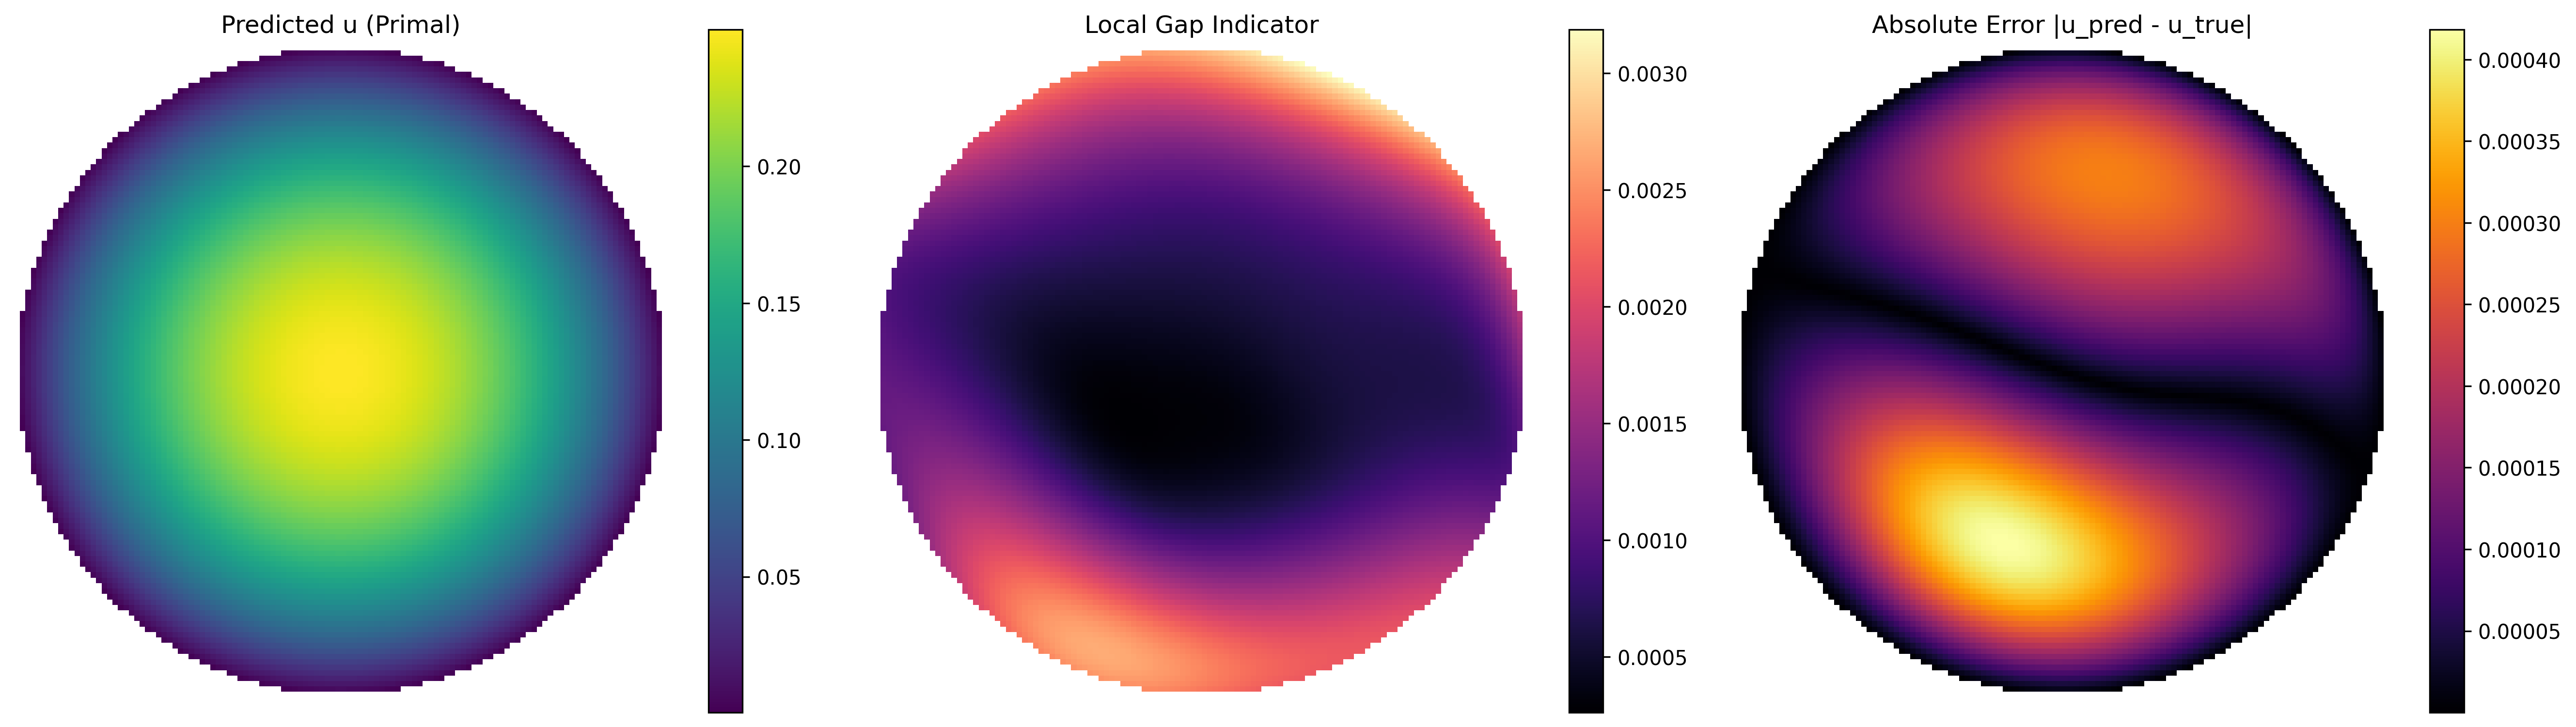
\includegraphics[width=\linewidth]{../exp/disk/HypoLoss.png}
      \end{center}
    \end{column}
  \end{columns}
\end{frame}

% ====================================================
% SLIDE 14 – Results: L-Shaped Domain
% ====================================================
\begin{frame}{Results: L-shaped Sector (Singular Solution)}

  \textbf{Training:} 10\,000 samples, 10\,001 epochs, Adam ($\text{lr}=10^{-3}$),
  float64, $2\!\to\!80\!\to\!80\!\to\!1$ networks, CPU.

  \medskip
  \begin{center}
  \renewcommand{\arraystretch}{1.3}
  \begin{tabular}{lrrrrr}
    \toprule
    \textbf{Method} & \textbf{Time (s)} & $G^2$ & $P^2$ & $D^2$
      & $\mathcal{E}_{\text{id}}$ \\
    \midrule
    Separate
      & 501.22 & $1.01\!\times\!10^{-1}$ & $9.24\!\times\!10^{-2}$
      & $8.81\!\times\!10^{-3}$ & $1.99\!\times\!10^{-5}$ \\
    Hypo, w/o mask
      & 181.88 & $3.72\!\times\!10^{-3}$ & $2.92\!\times\!10^{-3}$
      & $8.94\!\times\!10^{-4}$ & $8.99\!\times\!10^{-5}$ \\
    \textbf{Hypo, w/ $r^{2/3}$}
      & 191.54 & $\mathbf{1.13\!\times\!10^{-3}}$ & $\mathbf{4.03\!\times\!10^{-4}}$
      & $\mathbf{7.28\!\times\!10^{-4}}$ & $7.24\!\times\!10^{-7}$ \\
    \bottomrule
  \end{tabular}
  \end{center}

  \medskip
  \begin{columns}[T]
    \begin{column}{0.55\textwidth}
      \begin{alertblock}{Key findings}
        \begin{itemize}
          \item Joint training vs separate:
                \textbf{27$\times$ improvement} in $G^2$
                ($10^{-1} \to 3.72\!\times\!10^{-3}$)
          \item Adding $r^{2/3}$ mask:
                additional \textbf{7.2$\times$} reduction in $P^2$
          \item Hypotenuse bound remains \textbf{strict}:
                $G^2 = P^2 + D^2$ to $\mathcal{E}_{\text{id}} \sim 10^{-7}$
          \item Hypotenuse \textbf{2.6$\times$ faster}
                than separate training (191 s vs 501 s)
        \end{itemize}
      \end{alertblock}
    \end{column}
    \begin{column}{0.42\textwidth}
      \begin{center}
        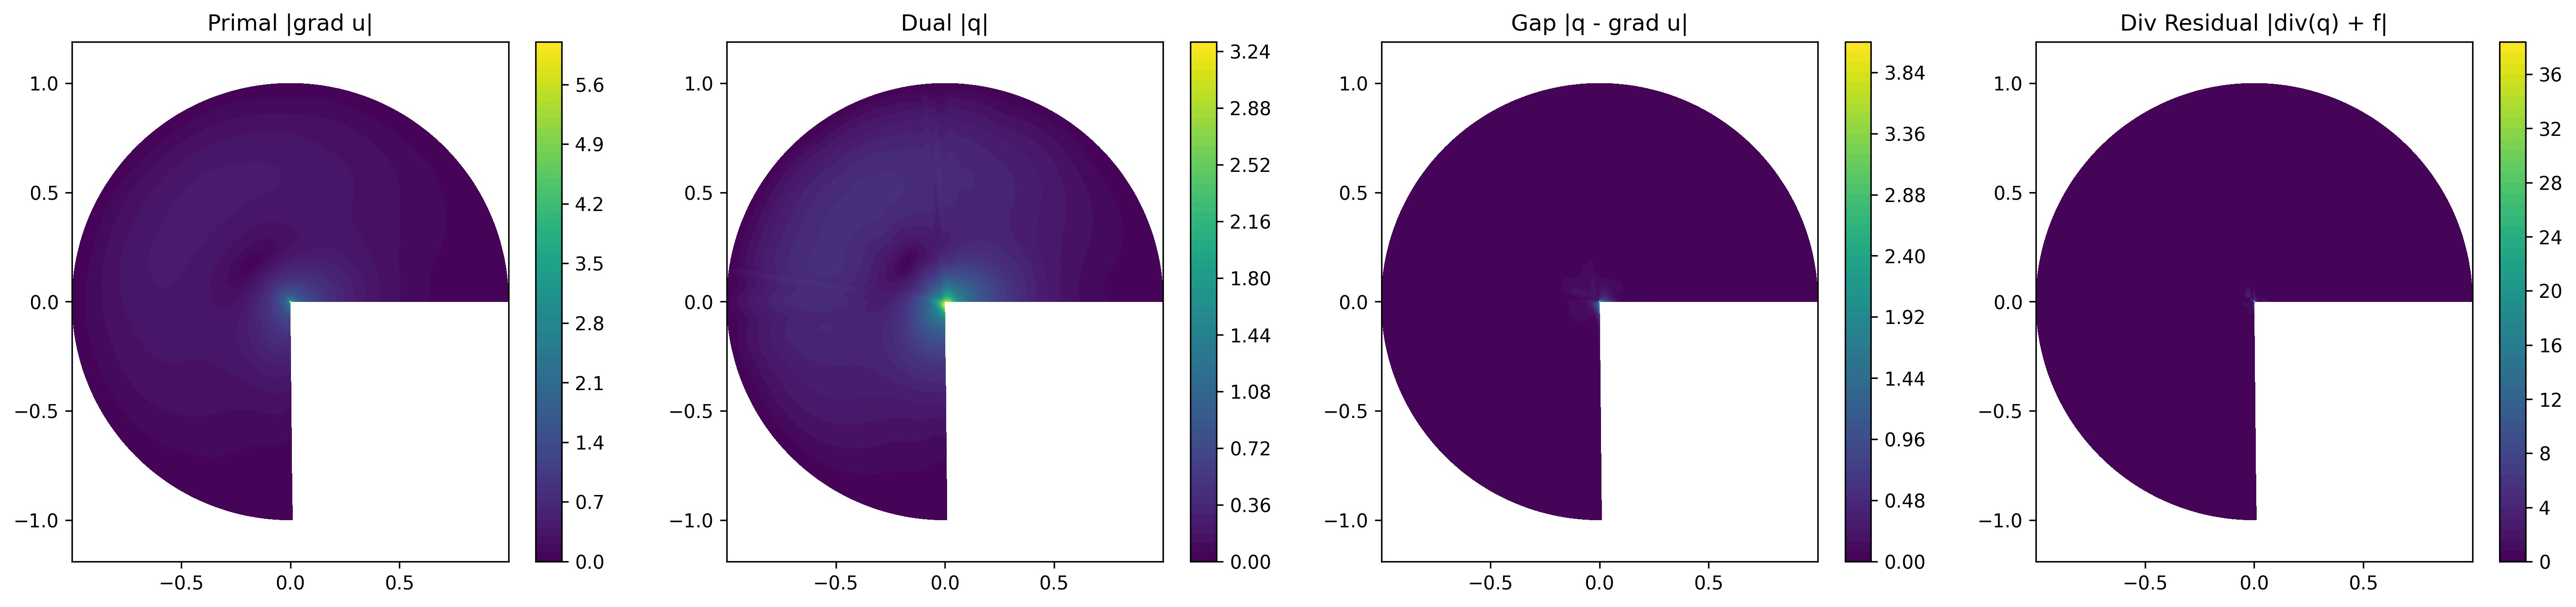
\includegraphics[width=\linewidth]{../exp/sector/hypo_general_dual.png}
      \end{center}
    \end{column}
  \end{columns}
\end{frame}

% ====================================================
\section{Summary}
% ====================================================

% ====================================================
% SLIDE 15 – Contributions
% ====================================================
\begin{frame}{Summary of Contributions}

  \begin{columns}[T]
    \begin{column}{0.48\textwidth}
      \begin{block}{1. Strictly Admissible Architectures}
        \begin{itemize}
          \item Distance mask $\Rightarrow$ exact BC ($v \in \mathcal{K}$)
          \item Curl operator $\Rightarrow$ exact $\divg\mathbf{p}=-f$
                ($\mathbf{p} \in \mathcal{S}$)
          \item Hard constraints, no penalty terms
        \end{itemize}
      \end{block}
      \medskip
      \begin{block}{2. Hypotenuse Loss}
        \begin{itemize}
          \item First-order only: no $\Delta v$ needed
          \item Certified upper bound $G^2 \ge P^2,\, D^2$
          \item Joint training: faster \& more accurate
        \end{itemize}
      \end{block}
    \end{column}
    \begin{column}{0.48\textwidth}
      \begin{block}{3. Singularity Enrichment}
        \begin{itemize}
          \item Asymptotic theory: $u \sim r^{\pi/\omega}$
          \item Explicit $r^{2/3}$ factor in trial space
          \item 7.2$\times$ improvement in primal error
        \end{itemize}
      \end{block}
      \medskip
      \begin{block}{Future Directions}
        \begin{itemize}
          \item 3-D: vector potentials for curl
          \item Adaptive sampling guided by local gap
          \item Extension to elasticity, Maxwell
          \item Automatic $\mathbf{p}_p$ construction
                for general $f$
        \end{itemize}
      \end{block}
    \end{column}
  \end{columns}

  \medskip
  \begin{center}
    \small
    \textbf{Code:}
    \url{https://github.com/ShengYaooo/Strict-Error-Control-in-Physics-Informed-Neural-Networks-via-the-Hypercircle-Method}
    \quad (commit \texttt{727e802})
  \end{center}
\end{frame}

% ====================================================
% SLIDE 16 – Thank you
% ====================================================
\begin{frame}[plain]
  \begin{center}
    \vspace{1.5cm}
    {\LARGE \textbf{Thank You}}\\[1cm]
    {\large Xuefeng Liu}\\[0.3cm]
    {\normalsize TWCU}\\[0.8cm]
    {\normalsize
      \emph{In collaboration with:} PingTing Hsieh \& ShengYao Huang (NCKU)}\\[1.2cm]
    \textbf{Hypercircle Identity:}
    \[
      \underbrace{\norm{\nabla v - \mathbf{p}}^2}_{\text{computable gap}}
      \;=\;
      \norm{\nabla v - \nabla u}^2 + \norm{\mathbf{p} - \nabla u}^2
    \]
  \end{center}
\end{frame}

\end{document}
